\documentclass[border=0.5mm]{standalone}

\usepackage{import}
\subimport{../../../}{preamble.tex}

\usepackage{tikz}
\usetikzlibrary{calc}

\usepackage{pgfplots}
\usepgfplotslibrary{fillbetween}

\begin{document}

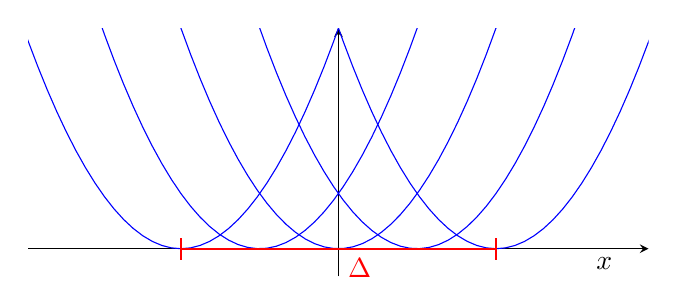
\begin{tikzpicture}

  \begin{axis}[
    ticks=none,
    axis lines=center,
    y=0.7cm,            % y unit vector
    x=1cm,            % x unit vector
    clip=true,
    ymax=4,
    ymin=-0.5,
    xlabel={ $x$},
    ylabel={},
    x label style={at={(axis description cs:0.9,0.05)},anchor=west},
    y label style={at={(axis description cs:0.22,0.85)},rotate=-90,anchor=south west},
    ]
    
    \foreach \a in {-2, ..., 2}{
      \addplot[mark=none, blue, samples=100, domain=-6:6] { (x-\a)^2 };
    }

    \draw[red, thick] (axis cs:-2,0) -- (axis cs:2,0);
    \draw[red, thick] (axis cs:-2,-0.2) -- (axis cs:-2,0.2);
    \draw[red, thick] (axis cs:2,-0.2) -- (axis cs:2,0.2);

    \node[above right] at (axis cs:0,-0.7) {{\color{red}$\Delta$}};
    
  \end{axis}
  
\end{tikzpicture}

\end{document}

%%% Local Variables:
%%% mode: latex
%%% TeX-master: t
%%% End:
